%%%%%%%%%%%%%%%%%%%%%%%%%%%%%%%%%%%%%%%%%
% a0poster Portrait Poster
% LaTeX Template
% Version 1.0 (22/06/13)
%
% The a0poster class was created by:
% Gerlinde Kettl and Matthias Weiser (tex@kettl.de)
% 
% This template has been downloaded from:
% http://www.LaTeXTemplates.com
%
% License:
% CC BY-NC-SA 3.0 (http://creativecommons.org/licenses/by-nc-sa/3.0/)
%
%%%%%%%%%%%%%%%%%%%%%%%%%%%%%%%%%%%%%%%%%

%----------------------------------------------------------------------------------------
%	PACKAGES AND OTHER DOCUMENT CONFIGURATIONS
%----------------------------------------------------------------------------------------

\documentclass[a0,portrait]{a0poster}

\usepackage{multicol} % This is so we can have multiple columns of text side-by-side
\columnsep=100pt % This is the amount of white space between the columns in the poster
\columnseprule=3pt % This is the thickness of the black line between the columns in the poster

\usepackage[svgnames]{xcolor} % Specify colors by their 'svgnames', for a full list of all colors available see here: http://www.latextemplates.com/svgnames-colors

\usepackage{times} % Use the times font
%\usepackage{palatino} % Uncomment to use the Palatino font

\usepackage{graphicx} % Required for including images
\graphicspath{{figures/}} % Location of the graphics files
\usepackage{booktabs} % Top and bottom rules for table
\usepackage[font=small,labelfont=bf]{caption} % Required for specifying captions to tables and figures
\usepackage{amsfonts, amsmath, amsthm, amssymb} % For math fonts, symbols and environments
\usepackage{wrapfig} % Allows wrapping text around tables and figures
\usepackage{hyperref}

\begin{document}

%----------------------------------------------------------------------------------------
%	POSTER HEADER 
%----------------------------------------------------------------------------------------

% The header is divided into two boxes:
% The first is 75% wide and houses the title, subtitle, names, university/organization and contact information
% The second is 25% wide and houses a logo for your university/organization or a photo of you
% The widths of these boxes can be easily edited to accommodate your content as you see fit

\begin{minipage}[b]{0.75\linewidth}
\veryHuge \color{NavyBlue} \textbf{K plus proches voisins (KNN)} \color{Black}\\ % Title
\Huge\textit{fiche d'aide}\\[2cm] % Subtitle
\huge Arts et Metiers\\[0.4cm] % University/organization
\\
\end{minipage}
%
\begin{minipage}[b]{0.25\linewidth}

\includegraphics[width=20cm]{logo.png}\\
\end{minipage}

\vspace{1cm} % A bit of extra whitespace between the header and poster content

%----------------------------------------------------------------------------------------

% \begin{multicols}{1} % This is how many columns your poster will be broken into, a portrait poster is generally split into 2 columns

%----------------------------------------------------------------------------------------
%	ABSTRACT
%----------------------------------------------------------------------------------------



%----------------------------------------------------------------------------------------
%	INTRODUCTION
%----------------------------------------------------------------------------------------

\color{SaddleBrown} % SaddleBrown color for the introduction

\section*{A quoi sert l'algorithme ?}

L'algorithme des k plus proches voisins (KNN) est utilisé à la fois pour la classification et la régression dans l'apprentissage supervisé. Ses applications incluent la classification d'images, la recommandation, la détection d'anomalies, la prédiction de valeurs, le traitement du signal, la cartographie, l'apprentissage semi-supervisé et la compression de données. KNN est particulièrement utile lorsque les données sont réparties de manière locale et que des informations provenant de voisins proches peuvent être utilisées pour prendre des décisions.
%----------------------------------------------------------------------------------------
%	OBJECTIVES
%----------------------------------------------------------------------------------------

\color{DarkSlateGray} % DarkSlateGray color for the rest of the content

\section*{Comment fonctionne le KNN ?}

L'algorithme des k plus proches voisins fonctionne en mesurant la proximité spatiale d'un nouvel exemple à k voisins les plus proches dans un ensemble de données existant. Il attribue au nouvel exemple une classe majoritaire parmi ses voisins pour la classification, ou prédit une valeur moyenne pour la régression. KNN est simple à comprendre, mais le choix de la distance et du nombre de voisins (k) peut influencer les résultats. Cet algorithme est utilisé pour des tâches de classification, de régression, de recommandation et de détection d'anomalies.

\begin{center}\vspace{1cm}
    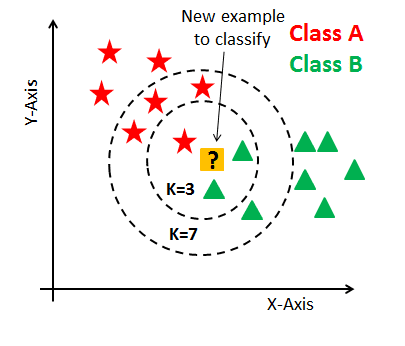
\includegraphics[width=0.3\linewidth]{knn.png}
    \captionof{figure}{classification d'un element par knn}
\end{center}

%----------------------------------------------------------------------------------------
%	MATERIALS AND METHODS
%----------------------------------------------------------------------------------------

\section*{Avantages et Inconvenients}

%------------------------------------------------

\subsection*{Avantages}

\begin{enumerate}
    \item Facile à comprendre et à implémenter
    \item Une fois entraîné, il ne nécessite pas de réentrainement lors de la modification de données
    \item Classification et régression
\end{enumerate}

\subsection*{Inconvenients}

\begin{enumerate}
    \item Sensible aux valeurs aberrantes
    \item Demande beaucoup de ressources pour calculer la distance entre les points
    \item Besoin de beaucoup de stockage pour les données
    \item Choix de k qui influe sur les résultats
    \item Ne fonctionne pas bien avec des données de grande dimension
\end{enumerate}

%----------------------------------------------------------------------------------------
%	RESULTS 
%----------------------------------------------------------------------------------------

\section*{Exemple}

On cherche à savoir si un fruit est une pomme ou une orange en fonction de son poids et de son diamètre. On a les données suivantes :

\begin{center}\vspace{1cm}
    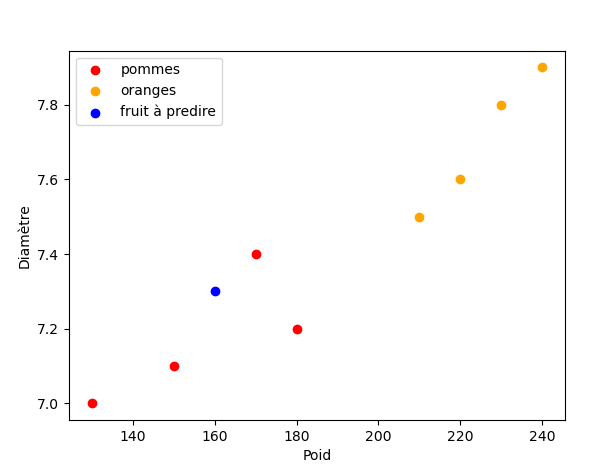
\includegraphics[width=0.4\linewidth]{knn2.png}
\end{center}

ici, l'algorithme renvoie que le fruit est une pomme.

%----------------------------------------------------------------------------------------
%	CONCLUSIONS
%----------------------------------------------------------------------------------------

\color{DarkSlateGray} % Set the color back to DarkSlateGray for the rest of the content


%----------------------------------------------------------------------------------------
%	ACKNOWLEDGEMENTS
%----------------------------------------------------------------------------------------

\section*{Pour aller plus loin}

\begin{enumerate}
    \item \href{https://scikit-learn.org/stable/auto_examples/linear_model/plot_ols.html}{Scikit-learn}.
    \item \href{https://en.wikipedia.org/wiki/Linear_regression.}{Wikipedia}
\end{enumerate}

%----------------------------------------------------------------------------------------

%\end{multicols}
\end{document}